\section{Progettazione controllore PID con desaturatore}
\label{sec:PIDdesaturatore}

	In questa sessione si procede alla progettazione del controllore PID con desaturatore. 
	
	
	
	
	
	
	
	
	
	
	
	
	\subsection{Il controllore PID}
	\label{subsec:introduzionePID}
	
		Un controllore PID utilizza tre diverse azioni: proporzionale, integrativa e derivativa. Nella sua configurazione
		più comune esse agiscono in parallelo, cioè sono alimentate dallo stesso ingresso e le tre uscite sono poi sommate
		per ottenere l'uscita complessiva del controllore, come in Figura \ref{fig:schemaPID}. Si noti che il blocco derivatore non è un semplice $s$, ma una funzione di trasferimento strettamente propria, altrimenti impossibile da realizzare. 
	
		\begin{figure}[H]
			\centering
			\begin{tikzpicture}[auto, node distance=1.6cm,>=latex']
			
				\node [input, name=input] {};
				\node [input, name=dirama, right of=input] {};
				\node [block, right of=dirama] (kI) {$K_I$};
				\node [block, above of=kI] (kP) {$K_P$};
				\node [block, below of=kI] (kD) {$K_D$};
				\node [block, right of=kI] (I) {$\frac{1}{s}$};
				\node [block, right of=kD] (D) {$\frac{s}{1+\tau_Ls}$};
				\node [sum, right of=I] (sum) {};
				\node [output, name=output, right of=sum] {};
			
				\draw [-] (input) -- node[pos=0.05] {$e(t)$} (dirama) {};
			
				\draw [->] (dirama) |- (kP) {};
				\draw [->] (dirama) -- (kI) {};
				\draw [->] (dirama) |- (kD) {};
			
				\draw [->] (kI) -- (I) {};
				\draw [->] (kD) -- (D) {};
			
				\draw [->] (kP) -| (sum) {};
				\draw [->] (I) -- (sum) {};
				\draw [->] (D) -| (sum) {};	
			
				\draw [->] (sum) -- node[pos=0.95] {$u(t)$} (output) {};
	
			\end{tikzpicture}
			\caption{Schema a blocchi di un controllore PID}
			\label{fig:schemaPID}
		\end{figure}
	
		\noindent La funzione di trasferimento del controllore può essere scritta come:
	
		\begin{empheq}[box=%
		\fbox]{equation}
			C(s) = K_P + \frac{K_I}{s} + \frac{K_D s}{1 + \tau _L s}
			\label{eq:PID}		
		\end{empheq}
	
		\noindent in cui sono presenti quattro parametri:
		\begin{itemize}
			\item $K_P$: costante dell'azione proporzionale
			\item $K_I$: costante dell'azione integrale
			\item $K_D$: costante dell'azione derivativa
			\item $\tau_L$: costante temporale legata all'azione derivativa
		\end{itemize}
	
		\noindent Si noti che in generale non è necessario utilizzare tutte e tre le azioni. Ognuna di esse infatti ha specifici effetti sulle prestazioni e sulla stabilità del sistema, schematizzate a seguire.
	
		\begin{figure}[H]
			\centering
			\begin{tikzpicture}[auto, node distance=1.6cm,>=latex']
		
				\node [input, name=input] {};
				\node [sum, right of=input] (sum) {};
				\node [block, right of=sum] (C) {$C(s)$};
				\node [block, right of=C] (P) {$P(s)$};
				\node [output, name=dirama, right of=P] {};
				\node [output, name=output, right of=dirama]  {};
				\node [output, name=fittizio, below of=C] {};
			
				\draw [->] (input) -- node[pos=0.05] {$r(t)$} node[pos=0.91] {$+$} (sum) {}; 
				\draw [->] (sum) -- (C) {};
				\draw [->] (C) -- node[pos=0.5] {$u(t)$} (P) {};
				\draw [-] (P) -- (dirama) {};
				\draw [->] (dirama) -- node[pos=0.95] {$y(t)$} (output) {};
			
				\draw [-] (dirama) |- (fittizio) {};
				\draw [->] (fittizio) -| node[pos=0.95] {$-$} (sum) {};
		
			\end{tikzpicture}
			\caption{Schema a blocchi di un classico controllo in retroazione}
			\label{fig:retroazione}
		\end{figure}
	
		\noindent Analizziamo ora gli effetti che le tre azioni del controllore portano, sia gli aspetti positivi che quelli negativi. In figura \ref{fig:retroazione} è schematizzato un classico sistema di controllo in retroazione. Definendo $G(s)=C(s)P(s)$ la funzione di trasferimento in catena aperta del sistema possiamo calcolare
	
		\begin{itemize}
			\item $\omega_a$: pulsazione di attraversamento, ovvero la pulsazione tale per cui il modulo di $G(s)$ raggiunge il valore uno;
			\item $m_{\phi}^G=180°+\arg[G(j\omega_a)]$: margine di fase, che a meno di sistemi sfortunati, da una  indicazione del grado di stabilità del sistema. Ovvero maggiore è il margine di fase, più stabile è il sistema.		 
		\end{itemize}
		
		\paragraph{Azione proporzionale P} 
	   	\label{par:P}
	   		\leavevmode\newline
	   		La parte proporzionale può essere scritta come 
	   		
	   		\begin{equation*}
	   			C_P(s)=K_P
	   		\end{equation*}
	   		
	   		\noindent Ciò porta ad avere dei diagrammi di Bode piatti, di ampiezza $20\log_{10}K_P$ dB per quanto riguarda il modulo e 0 per la fase. Questo significa che può modificare la pulsazione di attraversamento ma non il margine di fase.
	   		
	   	\paragraph{Azione integrale I}
	   	\label{par:I}
	   		\leavevmode\newline
	   		La parte integrale è invece
	   		
	   		\begin{equation*}
		   		C_I(s)=\frac{K_I}{s}
	   		\end{equation*}	
	   		
	   		\noindent Il modulo è una retta con intercetta con le ordinate pari a $20\log_{10}K_I$ dB e pendenza $-20$ dB/decade, e la fase una retta di ampiezza $-90°$. E' quindi rischioso da usare perché tende a far diventare il sistema $G(s)$ instabile, però offre il vantaggio di aggiungere un polo nell'origine e quindi di portare l'errore a regime a zero.
	   		
	   	\paragraph{Azione derivativa D}
	   	\label{par:D}
	   		\leavevmode\newline
	   		L'azione derivativa è invece
	   		
	   		\begin{equation*}
	   			C_D(s)=K_Ds
	   		\end{equation*} 
	   		
	   		\noindent In questo caso il modulo è una retta sempre con intercetta $20\log_{10}K_D$ ma con pendenza $20$ dB/decade, mentre la fase è una retta di altezza $90°$. La fase tende a far migliorare la stabilità, però la derivata del segnale amplifica il rumore in ingresso. E' necessario inoltre dire che un controllore così costruito risulta impossibile da progettare in pratica, perché avrebbe il modulo che cresce all'infinito. Quello che si fa è di aggiungere un polo in alta frequenza, facendo diventare il controllore
	   		
	   		\begin{equation*}
	   			D_D(s)=\frac{K_Ds}{1+\tau_Ls}
	   		\end{equation*} 	 
	
		\noindent I pregi e difetti delle tre azioni sono schematizzati nella tabella che segue.	
	
	
		\begin{table}[H]
			\begin{tabularx}{\textwidth}{|>{\setlength\hsize{0.6\hsize}\setlength\linewidth{\hsize}}X|>{\setlength\hsize{1.3\hsize}\setlength\linewidth{\hsize}}X|>{\setlength\hsize{1.1\hsize}\setlength\linewidth{\hsize}}X|}
			\hline
			\multicolumn{3}{|c|}{Classificazione dei tre termini del controllore in base ai pro e contro.}\\
			\hline
			Termine & Pro & Contro \\
			\hline
			\vphantom{1. Proporzionale}
			\vphantom{1. Proporzionale}
			1. Proporzionale &
			\vphantom{1. Proporzionale}
				\begin{itemize}
					\item Permette di modificare $\omega_a$ di $G(s)$ 
					\item Semplice
				\end{itemize} &
				\vphantom{1. Proporzionale}
				\begin{itemize}
					\item Non può modificare $m_\phi^G$
				\end{itemize}\\
				\hline
				\vphantom{2. Integrale}
				\vphantom{2. Integrale}
				2. Integrale &
				\vphantom{2. Integrale}
				\begin{itemize}
					\item Elimina l'errore a regime
					\item Elimina disturbi costanti in ingresso
				\end{itemize} &
				\vphantom{2. Integrale}
				\begin{itemize}
					\item Rende il sistema più instabile
				\end{itemize}\\
				\hline
				\vphantom{3. Derivativo}
				\vphantom{3. Derivativo}
				3. Derivativo &
				\vphantom{3. Derivativo}
				\begin{itemize}
					\item Rende il sistema più stabile
				\end{itemize} &
				\vphantom{3. Derivativo}
				\begin{itemize}
					\item Amplifica rumori di misura
				\end{itemize}\\
				\hline
			\end{tabularx}
			\label{tab:ProContro}
		\end{table}
	
	
	
	
	
	
	
	
	
	
	
	
	
	
	
	
	
	
	\subsection{Progettazione in frequenza del controllore PID}
	\label{sub:ProgettazionePID}
	
		Possiamo riscrivere l'equazione del PID come
		
		\begin{equation}
			C(s)=K_P + \frac{K_I}{s} + K_Ds=\frac{K_Ps+K_I+K_Ds^2}{s}=\frac{K_I(1+\frac{K_P}{K_I}s+\frac{K_D}{K_I}s^2)}{S}
			\label{eq:PIDriscritto}
		\end{equation}
		
		\noindent e definendo $\tau_I=\frac{K_P}{K_I}$ il tempo dell'azione integrale ,$\tau_D=\frac{K_D}{K_P}$ il tempo dell'azione derivativa e nell'ipotesi che $\tau_I>>\tau_D$ \footnote{Questa ipotesi è del tutto lecita, perché l'azione integrale ha appunto bisogno che l'integrale del segnale raggiunga valori significativi prima di intervenire. Mentre l'azione derivativa, soprattutto in un ingresso a gradino, agisce istantaneamente.} si ottiene 
		
		\begin{equation}
			C(s)=\frac{K_I}{s}\bigl(1+\tau_Is+\tau_D\tau_Is^2\bigl) \approx \frac{K_I}{s}\bigl(1+\tau_Is\bigl)\bigl(1+\tau_Ds\bigl)
			\label{eq:PIDtau}
		\end{equation}
		
		\noindent Aggiungendo in fine il termine di non idealità $\tau_L$ della parte derivativa e nell'ulteriore ipotesi che $\tau_I>>\tau_D>>\tau_L$ \footnote{Anche questa ipotesi è lecita, visto che il polo si cerca di metterlo più in alta frequenza possibile.}
		
		\begin{equation}
			C(s) \approx \frac{K_I(1+\tau_Is)(1+\tau_Ds)}{s(1+\tau_Ls)}
			\label{eq:PIDfinale}
		\end{equation}
	
		\noindent Perché il controllore dia i benefici desiderati, bisogna che sia soddisfatta la condizione $\tau_I>>\tau_D>>\frac{1}{\omega_a^{min}}>>\tau_L$ dove $\omega_a^{min}$ rappresenta la minima pulsazione di attraversamento richiesta nelle specifiche. Ciò comporta a scegliere
		
		\begin{empheq}[box=%
		\fbox]{equation}
			\tau_L=\alpha\frac{1}{\omega_a^{min}} \singleSpacing, \trippleSpacing \frac{1}{3}\le\alpha\le\frac{1}{10}
			\label{eq:tauL}
		\end{empheq}
		
		\noindent Si definisce poi 
		\begin{equation}
			a=\frac{1}{|P(j\omega_a)|} \trippleSpacing \trippleSpacing \trippleSpacing \theta=\arg\bigl[C(j\omega_a)\bigl]=m_{\phi}^G-180°-\arg\bigl[P(j\omega_A)\bigl]
		\end{equation}
	
		\noindent e riscrivendo la funzione di trasferimento del controllore nella variabile $j\omega$
		
		\begin{equation}
			C(j\omega_a)=K_P-j\frac{K_I}{\omega_a}+j\omega_aK_D=K_P+j\bigl(\omega_aK_D-\frac{K_I}{\omega_a}\bigl)
		\end{equation}
		
		\noindent si ottiene
		
		\begin{align}
			\Re\Bigl[C(j\omega_a)\Bigl] &= a\cos\theta=K_P \\
			\Im\Bigl[C(j\omega_a)\Bigl] &= a\sin\theta=\omega_aK_D-\frac{K_I}{\omega_a}
			\label{eq:asen}
		\end{align}
	
		\noindent L'equazione \ref{eq:asen} mi fornisce un grado di libertà nella scelta dei parametri $K_P$ e $K_D$, tenendo però conto di soddisfare $\tau_I>>\tau_D$. Solitamente si sceglie 
		
		\begin{equation}
			\tau_I=b\tau_D \singleSpacing, \trippleSpacing b\ge4
		\end{equation}
	
		\noindent stando attenti a non scegliere $b$ troppo grande, altrimenti avrei tempi di reiezione del disturbo troppo lunghi. Rimane solo da ricavare $K_I$, per fare ciò basta risolvere l'equazione
		
		\begin{equation}
			K_Ia\sin\theta=\omega_a\frac{K_P^2}{b}-\frac{K_I^2}{\omega_a}
		\end{equation}
	
		\noindent con $K_I$ incognita. Risolvendola si otterranno due valori, ma a noi interessa solo quello positivo e quindi
		
		\begin{equation}
			K_I=\frac{a\omega_a}{2}\Biggl[\sqrt{\sin^2\theta+\frac{4}{b}\cos^2\theta}-\sin\theta\Biggl]
		\end{equation}
		
		\noindent e allora
		
		\begin{equation}
			K_D=\frac{K_P^2}{bK_I}
		\end{equation}
		
		\noindent In questo caso però, le specifiche richieste non sono fornite in frequenza, ma in termini temporali. 
		
		\begin{align}
			t_s &\le 30 \singleSpacing \textrm{[s] rispetto a $\pm1$ [gradi] dal valore a regime} \\
			S   &\le 5 \singleSpacing \textrm{[gradi]}
			%r   &= 10,\singleSpacing 50, \singleSpacing 120 \singleSpacing \textrm{[gradi]} \\
			%d   &= \pm0.5 \singleSpacing \textrm{[Volt]}  
		\end{align}
		
		\noindent Il tempo di assestamento viene trasformato in un limite alla banda passante minima che il sistema deve garantire. Visto che si considera un sistema del secondo ordine, è possibile approssimare la banda passante con la frequenza di taglio $\omega_a$ e ottenere:
		
		\begin{equation}
			\omega_a^{min}= \frac{3}{\xi t_{s,max}}
		\end{equation}
		
		\noindent dove $\xi$ rappresenta il coefficiente di smorzamento. Il vincolo sul massima sovraelongazione invece può essere convertito in una richiesta sul minimo margine di fase $m_{\phi}$ ammissibile. Per la conversione si possono allora utilizzare i due grafici riportati in figura \ref{fig:mSxiS}. Per una spiegazione dettagliata su come si possono ricavare i due grafici è possibile consultare l'appendice \ref{app:sistemaSecondoordine}.
		
		\begin{figure}[H]
			\centering
			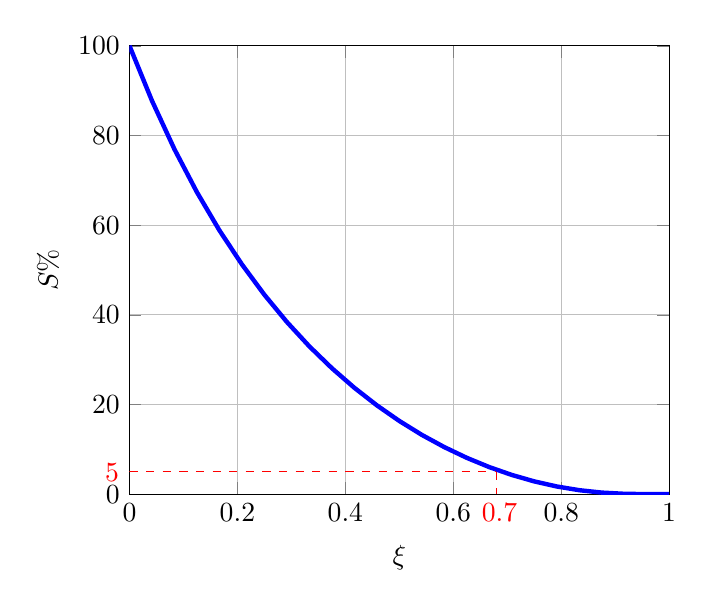
\begin{tikzpicture}[scale=1]
			    %\draw[help lines,step=.2] (0,0) grid (6,6);
				
				\begin{axis}[grid=both, xlabel=\phantom{$m_{\phi}^G$} $\xi$ \phantom{$m_{\phi}^G$}, ylabel=$S\singleSpacing \%$,enlargelimits=false]
			    	\addplot[domain=0:1, blue, ultra thick] {100*e^((-3.14*x)/(1-x^2)^(1/2)};
			    
			    	\addplot[red, dashed] coordinates {(0,5) (0.68,5)};
			    	\addplot[red, dashed] coordinates {(0.68,5) (0.68,0)};
				\end{axis}
				
				\node[red] at (-0.22,.28) {$5$};
				\node[red] at (4.7,-.24) {$0.7$};
			\end{tikzpicture}
			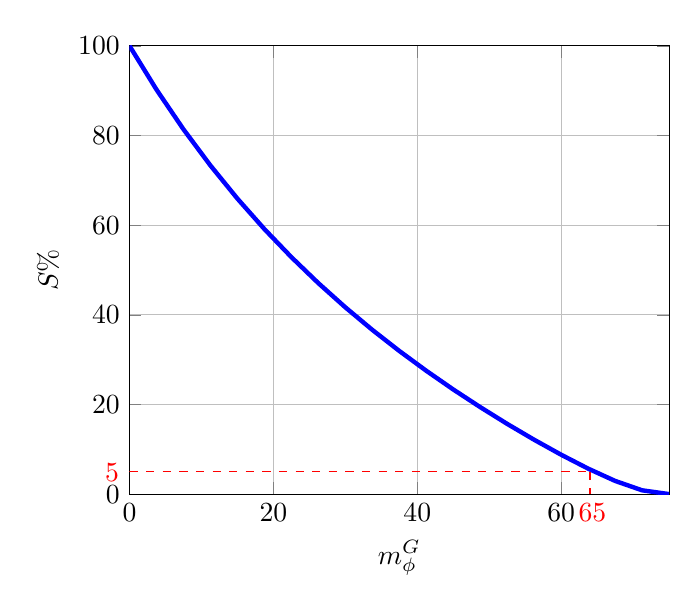
\begin{tikzpicture}[scale=1]
				%\draw[help lines,step=.2] (0,0) grid (6,6);
				\begin{axis}[grid=both, xlabel=$m_{\phi}^G$, ylabel=$S\singleSpacing \%$,enlargelimits=false]
			    	\addplot[domain=0:90, blue, ultra thick] {100*e^((-3.14*(tan(x)/(16*(tan(x))^2+16)^(1/4)))/((1-((tan(x)/(16*(tan(x))^2+16)^(1/4)))^2)^(1/2)))};
			    	
			    	\addplot[red, dashed] coordinates {(0,5) (64,5)};
			    	\addplot[red, dashed] coordinates {(64,5) (64,0)};
				\end{axis}
				
				\node[red] at (-0.22,.28) {$5$};
				\node[red] at (5.88,-.24) {$65$};
			\end{tikzpicture}
			\caption{Relazione tra $m_{\phi}$ e $S$ e tra $\xi$ e $S$.}
			\label{fig:mSxiS}
		\end{figure}
		
		
		
		
		
		
		
	
	
	
	
	
	
	
	
	
	
	
		
		
	\subsection{Progetto del controllore PID con desaturatore}
	\label{subsec:Desaturatore}
	
		\begin{figure}[H]
			\centering
			\begin{tikzpicture}[auto, node distance=1.6cm,>=latex']
				\node [input, name=input] {};
				\node [sum, right of=input] (sum1) {};
				\node [input, name=dirama1, right of=sum1] {};
				\node [block, right of=dirama1] (D) {$K_D\frac{s}{1+\tau_Ls}$};	
				\node [block, above of=D] (P) {$K_P$};
				\node [block, below of=D] (I) {$\frac{K_I}{s}$};
				\node [sum, below of=dirama1] (sum2) {};
				\node [sum, right of=D] (sum3) {};
				\node [input, name=dirama2, right of=sum3] (dirama2) {};
				\node [block, right of=dirama2] (saturatore) {saturatore};
				\node [input, name=dirama3, right of=saturatore] {};
				\node [block, right of=dirama3] (Ps) {$P(s)$};
				\node [input, name=dirama4, right of=Ps] {};
				\node [output, name=output, right of=dirama4] {};
				\node [sum, below of=dirama2] (sum4) {};
				\node [input, name=fittizio, below of=sum4] {};	
				\node [block, left of=fittizio] (Ka) {$K_a$};
				\node [input, name=fittizio2, below of=Ka] {};

				\draw [->] (input) --  node[pos=0.05] {$r(t)$}  node[pos=0.91] {$+$} (sum1) {};
				\draw [-] (sum1) --  node[pos=0.3] {$e(t)$} (dirama1) {};
				\draw [->] (dirama1) |- (P) {};
				\draw [->] (dirama1) -- (D) {};
				\draw [->] (dirama1) --  node[pos=0.95] {$+$} (sum2) {};
				\draw [->] (P) -| (sum3) {};
				\draw [->] (D) -- (sum3) {};
				\draw [->] (I) -| (sum3) {};
				\draw [->] (sum2) -- (I) {}; 
				\draw [-] (sum3) --  node[pos=0.5] {$u_{PID}(t)$} (dirama2) {};
				\draw [->] (dirama2) -- (saturatore) {};
				\draw [-] (saturatore) --  node[pos=0.6] {$u(t)$} (dirama3) {};
				\draw [->] (dirama3) -- (Ps) {};
				\draw [-] (Ps) -- (dirama4) {};
				\draw [->] (dirama4) --  node[pos=0.95] {$y(t)$} (output) {};
				\draw [->] (dirama2) --  node[pos=0.95] {$+$} (sum4) {}; 	
				\draw [-] (sum4) -- (fittizio) {};	
				\draw [->] (fittizio) -- (Ka) {};
				\draw [->] (Ka) -|  node[pos=0.95] {$-$} (sum2) {};
				\draw [->] (dirama3) |-  node[pos=0.95] {$-$} (sum4) {};	
				\draw [-] (dirama4) |- (fittizio2) {};
				\draw [->] (fittizio2) -|  node[pos=0.98] {$-$} (sum1) {};
			\end{tikzpicture}
			\caption{Schema a blocchi di un controllore PID con desaturatore}
			\label{fig:PIDdesaturatore}
		\end{figure}
	
		\noindent Il motore utilizzato in laboratorio è comandato con un segnale di tensione, tale segnale deve essere compreso tra un intervallo di valori pari a $[-5,5]$ Volt. Ciò significa che è necessario saturare il segnale di controllo con un dispositivo denominato saturatore. Saturando l'ingresso al motore, l'errore $e(t)$ che comanda il controllore tende a diminuire più lentamente e il suo integrale sarà allora maggiore. Questo vuol dire che amplifica l'azione integrale durante la saturazione, rendendo il sistema più instabile. Per ovviare a questo introduco un secondo controllo in retroazione che interviene solo in caso di saturazione, lo schema di tale controllo è presente in Figura \ref{fig:PIDdesaturatore}. Questa retroazione diminuisce il termine integrale per un fattore proporzionale alla differenza tra l'uscita del controllore e la vera uscita che riceve il motore. Rimane quindi da scegliere la variabile $K_a$. Con qualche passaggio algebrico è possibile scrivere la funzione di trasferimento tra l'uscita del controllore $U_{PID}(s)$ e l'errore $E(s)$ in presenza di saturazione come   
	
		\begin{equation}
			U_{PID}(s)=\frac{K_P+K_Ds+\frac{K_I}{s}}{1+\frac{K_aK_I}{s}}E(s)
			\label{eq:Upid}
		\end{equation}
	
		\noindent Si vede dall'equazione \ref{eq:Upid} che il parametro $K_a$ introduce un filtro passa basso che tende a rallentare il controllo. Allora si definisce la costante temporale del desaturatore $\tau_a=K_aK_I$ e quello che si vuole è che $\tau_a<t_s$. Tipicamente si sceglie
		
		\begin{empheq}[box=%
		\fbox]{equation}
			\tau_a \approx \frac{1}{3}t_s \trippleSpacing \Rightarrow \trippleSpacing K_a \approx \frac{1}{3t_sK_I}
		\end{empheq}